
\chapter{Tools holding registers}

Per pilotare singoli bit o singole byte/word di holding registers
sono presenti alcuni tools 
accessibili dal menu a tendina
"Tool registers". I tool seguenti si applicano solo a holding register, 
sono utilizzati principalmente per
pilotare su PLC oggetti di tipo \%MX,\%MB,\%MW:

\section{Tool comandi bit}

\begin{figure}[H]
\centering
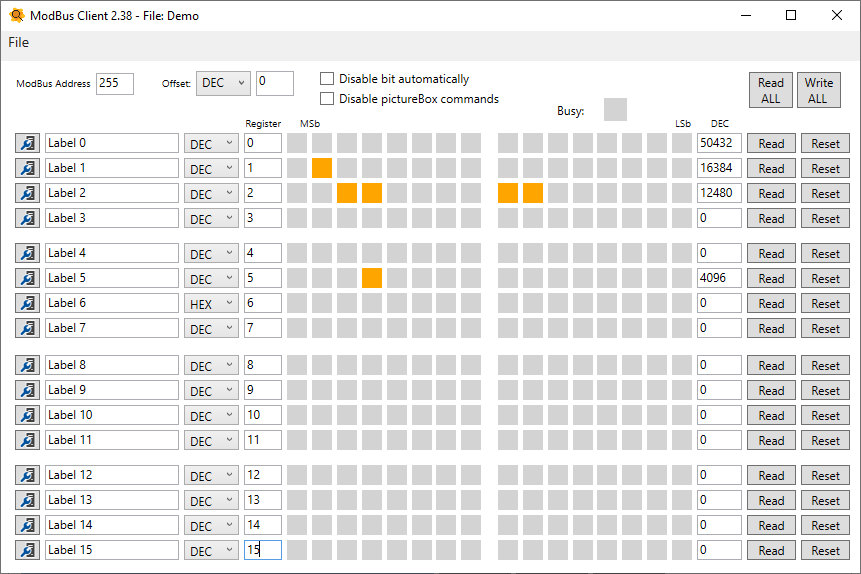
\includegraphics[width=0.85\textwidth]{../Img/Tool_Command_Bit.PNG}
\caption{Tool comandi bit}
\label{holding_main_win}
\end{figure}

Nella finestra Tool command bit è possibile leggere e visualizzare i registri nei singoli bit
che li compongono. Premendo sul singolo bit è possibile invertirne lo stato
(di default lavorano come un "passo passo" altrimenti 
se è flaggata l'opzione "disabilita bit automaticamente" al click del mouse il bit è
forzato a 1 e successivamente a 0).
\newpage
Premendo i pulsanti a fianco delle etichette si apre la finestra visualizzata a seguire con
la quale è possibile dare un etichetta specifica ai singoli bit
all'interno di una word. Le etichette in questione
fanno riferimento solo alla finestra della pagina precedente, non vengono visualizzate nella tab 
"Holding registers FC 03" della finestra principale. 

\begin{figure}[H]
\centering
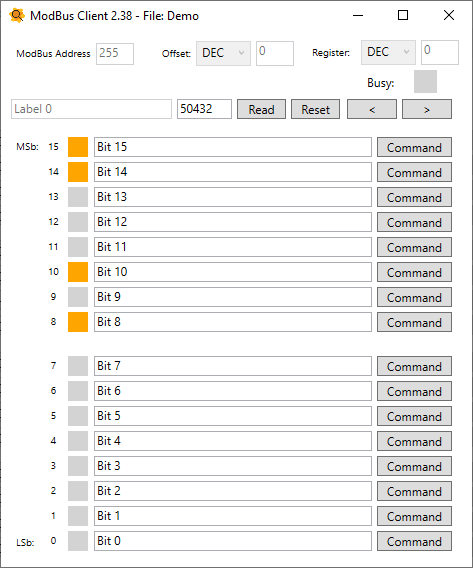
\includegraphics[width=0.55\textwidth]{../Img/Tool_Command_Bit_Label.PNG}
\caption{Tool comandi bit - Label Bits}
\end{figure}

Le etichette assegnate ai singoli bit diventano poi tooltip dei bit nella visualizzazione
principale riportata nell'immagine \ref{holding_main_win}. I pulsanti "<" e ">" in alto a destra permettono
di scorrere fra le word della finestra principale.

\section{Tool comandi byte}

\begin{figure}[H]
\centering
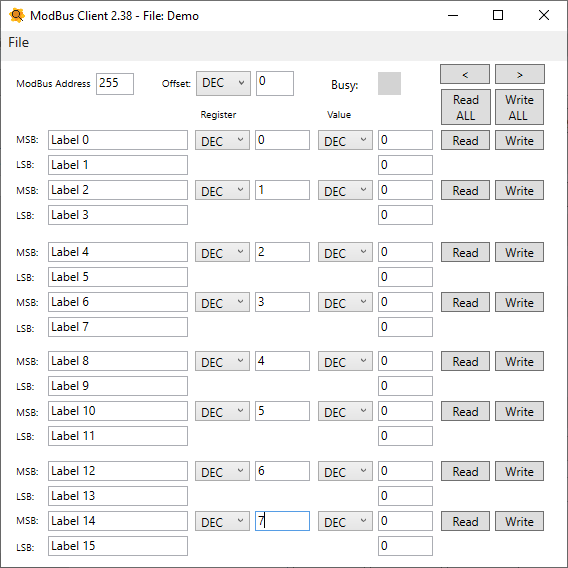
\includegraphics[width=0.55\textwidth]{../Img/Tool_Command_Byte.PNG}
\caption{Tool comandi byte}
\end{figure}

Dalla finestra riportata sopra è possibile inviare comandi ai singoli byte che verranno poi
scritti come singole word sul target. E' possibile creare finestre personalizzate con cui inviare
comandi a registri riferiti anche a posizioni diverse. I pulsanti "<" e ">" in alto a destra permettono
di scorrere fra 4 diversi profili della finestra.
Le celle scritte vengono colorate di verde mentre quelle lette di blu.

\section{Tool comandi word}

\begin{figure}[H]
\centering
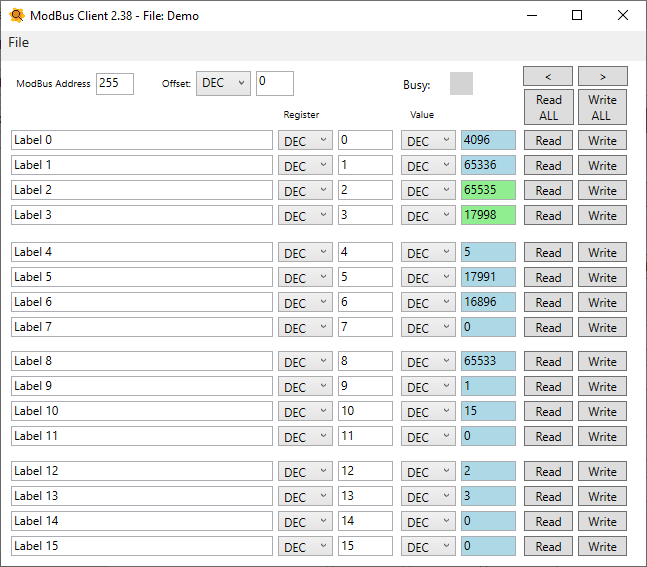
\includegraphics[width=0.55\textwidth]{../Img/Tool_Command_Word.PNG}
\caption{Tool comandi word}
\end{figure}

La finestra word contiene le stesse funzioni viste in precedenza per i singoli bytes, solo
divise per word. Come la precedente con i pulsanti "<" e ">" in alto a destra si può
scorrere fra 4 diversi profili della finestra.
Le celle scritte vengono colorate di verde mentre quelle lette di blu.
